%package list
\documentclass{article}
\usepackage[top=3cm, bottom=3cm, outer=3cm, inner=3cm]{geometry}
\usepackage{multicol}
\usepackage{graphicx}
\usepackage{url}
%\usepackage{cite}
\usepackage{hyperref}
\usepackage{array}
%\usepackage{multicol}
\newcolumntype{x}[1]{>{\centering\arraybackslash\hspace{0pt}}p{#1}}
\usepackage{natbib}
\usepackage{pdfpages}
\usepackage{multirow}
\usepackage[normalem]{ulem}
\useunder{\uline}{\ul}{}
\usepackage{svg}
\usepackage{xcolor}
\usepackage{listings}
\lstdefinestyle{ascii-tree}{
	literate={├}{|}1 {─}{--}1 {└}{+}1 
}
\lstset{basicstyle=\ttfamily,
	showstringspaces=false,
	commentstyle=\color{red},
	keywordstyle=\color{blue}
}
%\usepackage{booktabs}
\usepackage{caption}
\usepackage{subcaption}
\usepackage{float}
\usepackage{array}

\newcolumntype{M}[1]{>{\centering\arraybackslash}m{#1}}
\newcolumntype{N}{@{}m{0pt}@{}}


%%%%%%%%%%%%%%%%%%%%%%%%%%%%%%%%%%%%%%%%%%%%%%%%%%%%%%%%%%%%%%%%%%%%%%%%%%%%
%%%%%%%%%%%%%%%%%%%%%%%%%%%%%%%%%%%%%%%%%%%%%%%%%%%%%%%%%%%%%%%%%%%%%%%%%%%%
\newcommand{\itemEmail}{wchoquehuancab@unsa.edu.pe}
\newcommand{\itemStudent}{William Herderson Choquehuanca Berna}
\newcommand{\itemCourse}{Laboratorio de P web}
\newcommand{\itemCourseCode}{20233469}
\newcommand{\itemSemester}{III}
\newcommand{\itemUniversity}{Universidad Nacional de San Agustín de Arequipa}
\newcommand{\itemFaculty}{Facultad de Ingeniería de Producción y Servicios}
\newcommand{\itemDepartment}{Departamento Académico de Ingeniería de Sistemas e Informática}
\newcommand{\itemSchool}{Escuela Profesional de Ingeniería de Sistemas}
\newcommand{\itemAcademic}{2024 - A}
\newcommand{\itemInput}{Del 9 de mayo 2024}
\newcommand{\itemOutput}{Al 10 de mayo 2024}
\newcommand{\itemPracticeNumber}{03}
\newcommand{\itemTheme}{JavaScript}
%%%%%%%%%%%%%%%%%%%%%%%%%%%%%%%%%%%%%%%%%%%%%%%%%%%%%%%%%%%%%%%%%%%%%%%%%%%%
%%%%%%%%%%%%%%%%%%%%%%%%%%%%%%%%%%%%%%%%%%%%%%%%%%%%%%%%%%%%%%%%%%%%%%%%%%%%

\usepackage[english,spanish]{babel}
\usepackage[utf8]{inputenc}
\AtBeginDocument{\selectlanguage{spanish}}
\renewcommand{\figurename}{Figura}
\renewcommand{\refname}{Referencias}
\renewcommand{\tablename}{Tabla} %esto no funciona cuando se usa babel
\AtBeginDocument{%
	\renewcommand\tablename{Tabla}
}

\usepackage{fancyhdr}
\pagestyle{fancy}
\fancyhf{}
\setlength{\headheight}{30pt}
\renewcommand{\headrulewidth}{1pt}
\renewcommand{\footrulewidth}{1pt}
\fancyhead[L]{\raisebox{-0.2\height}{
\includegraphics[width=3cm]{img/logo_episunsa.png}}}
\fancyhead[C]{\fontsize{7}{7}\selectfont	\itemUniversity \\ \itemFaculty \\ \itemDepartment \\ \itemSchool \\ \textbf{\itemCourse}}
\fancyhead[R]{\raisebox{-0.2\height}{
\includegraphics[width=1.2cm]{img/logo_abet}}}
\fancyfoot[L]{Luis, Fernando, Anthony, William}
\fancyfoot[C]{\itemCourse}
\fancyfoot[R]{Página \thepage}

% para el codigo fuente
\usepackage{listings}
\usepackage{color, colortbl}
\definecolor{dkgreen}{rgb}{0,0.6,0}
\definecolor{gray}{rgb}{0.5,0.5,0.5}
\definecolor{mauve}{rgb}{0.58,0,0.82}
\definecolor{codebackground}{rgb}{0.95, 0.95, 0.92}
\definecolor{tablebackground}{rgb}{0.8, 0, 0}

\lstset{frame=tb,
	language=bash,
	aboveskip=3mm,
	belowskip=3mm,
	showstringspaces=false,
	columns=flexible,
	basicstyle={\small\ttfamily},
	numbers=none,
	numberstyle=\tiny\color{gray},
	keywordstyle=\color{blue},
	commentstyle=\color{dkgreen},
	stringstyle=\color{mauve},
	breaklines=true,
	breakatwhitespace=true,
	tabsize=3,
	backgroundcolor= \color{codebackground},
}

\begin{document}
	
	\vspace*{10px}
	
	\begin{center}	
		\fontsize{17}{17} \textbf{ Informe de Laboratorio \itemPracticeNumber}
	\end{center}
	\centerline{\textbf{\Large Tema: \itemTheme}}
	%\vspace*{0.5cm}	
	
	\begin{flushright}
		\begin{tabular}{|M{2.5cm}|N|}
			\hline 
			\rowcolor{tablebackground}
			\color{white} \textbf{Nota}  \\
			\hline 
			\\[30pt]
			\hline 			
		\end{tabular}
	\end{flushright}	
	
	\begin{table}[H]
		\begin{tabular}{|x{4.7cm}|x{4.8cm}|x{4.8cm}|}
			\hline 
			\rowcolor{tablebackground}
			\color{white} \textbf{Estudiantes} & \color{white}\textbf{Escuela}  & \color{white}\textbf{Asignatura}   \\
			\hline 
			{\itemStudent \par \itemEmail} & \itemSchool & {\itemCourse \par Semestre: \itemSemester \par Código: \itemCourseCode}     \\
			\hline 			
		\end{tabular}
	\end{table}		
	
	\begin{table}[H]
		\begin{tabular}{|x{4.7cm}|x{4.8cm}|x{4.8cm}|}
			\hline 
			\rowcolor{tablebackground}
			\color{white}\textbf{Laboratorio} & \color{white}\textbf{Tema}  & \color{white}\textbf{Duración}   \\
			\hline 
			\itemPracticeNumber & \itemTheme & 04 horas   \\
			\hline 
		\end{tabular}
	\end{table}
	
	\begin{table}[H]
		\begin{tabular}{|x{4.7cm}|x{4.8cm}|x{4.8cm}|}
			\hline 
			\rowcolor{tablebackground}
			\color{white}\textbf{Semestre académico} & \color{white}\textbf{Fecha de inicio}  & \color{white}\textbf{Fecha de entrega}   \\
			\hline 
			\itemAcademic & \itemInput &  \itemOutput  \\
			\hline 
		\end{tabular}
	\end{table}
	
	\section{Actividades}
	\begin{itemize}		
		\item Use la consola del browser para probar la sintaxis de JavaScript, pruebe declarar variables, arreglos, ciclos, condicionales, funciones flecha, funciones de alto orden.
		Cree una página  html y haga que esta ejecute un programa en JavaScript que esté en un archivo distinto.
	\end{itemize}
	\section{Ejercicios Propuestos}
	\begin{itemize}		
		\item Escriba una función que reciba el número de día de la fecha actual new Date()  y devuelva el texto del día de la semana correspondientes. Por ejemplo si recibe 0, devolvería “Domingo”.
		
		\item Escriba una página web que reciba un texto y al presionar un botón muestre el mismo texto invertido en otra sección (div). Por ejemplo si se escribe “Hola”, se mostraría como “aloH”.
		\item Escribir una página que muestre cuántos días faltan para el día de Arequipa!
		\item Escribir un página que reciba el URL de la sesión de google meet de hoy y devuelva el código de la sesión sin guiones separadores.
		\item Escribir una página que permita calcular la suma de todos los valores de una tabla de valores dinámica. La idea es crear una página web con un formulario que te permita decir cuantos valores tendrá la tabla, luego, al enviar el formulario la tabla se debe crear dinámica y aleatoriamente, junto con otro botón de envió para calcular la suma.
		\item Pagina1.html - Cree una página web con un texto y dos botones (al estilo del ejemplo del foco que se enciende y apaga) que permitan cambiar el tamaño de la letra de un texto, intente hacerlo también con los colores.
		\item Pagina2.html - Cree una página web que permita realizar las operaciones aritmética, lógicas y de bits básicas, de manera dinámica( se podrá elegir cualquier operador) y se trabajará con dos argumentos.
		\item Resolver los 67 ejercicios de javaScript en w3schools.com y subir un pantallazo con su nombre y apellido.
		La entrega de la tarea será usando git, para esto usted deberá usar GitHub para subir las distintas versiones de sus tareas (todos sus intentos), tendrá que compartir el proyecto privado con el profesor (CarloCorrales010) con permisos de administrador.  Por este medio entregará el enlace a su proyecto en github.
		La calificación tendrá los siguientes criterios:
		I. Las tareas que sean resueltas a última hora (en los últimos dos días de entrega) tendrá nota 11 como máximo.
		II. Deberá procurar subir al menos 1 versión de su tarea cada día
		III.  Cada línea mal sangrada (indent) restará 1 punto a su nota.
		
	\end{itemize}
	
	\section{Equipos, materiales y temas utilizados}
	\begin{itemize}
		\item Sistema operativo de 64 bits, procesador basado en x64.
		\item Latex. 
		\item git version 2.41.0.windows.1
		\item Lenguaje JavaScript.
		\item IDE Visual Sudio Code.
	\end{itemize}
	\section{URL Github, Video}
	\begin{itemize}
		\item URL del Repositorio GitHub para clonar o recuperar.
		\item \url{https://github.com/WilliamLawrence25/PWeb2/tree/main/Lab3}
		\item URL para el video flipgrid.
		\item \url{VIDEO EN PROGRESO}	
	\end{itemize}
	\clearpage	
	
	\section{Capturas de los ejercicios propuestos}
	
	\subsection{Ejercicio 1}
	\begin{figure}[H]
		\centering
		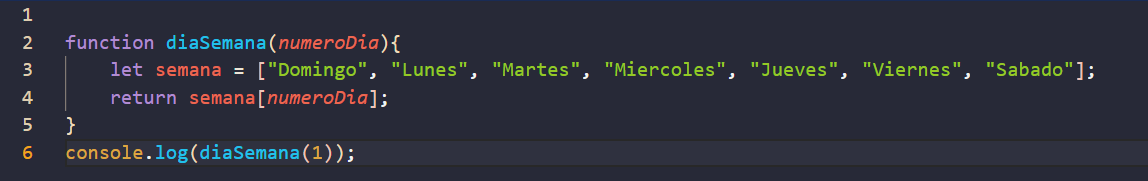
\includegraphics[width=1.0\textwidth, keepaspectratio]{img/ejercicio1b}
	\end{figure}
	
	\subsection{Ejercicio 2}
	\begin{itemize}
		\item HTML
	\end{itemize}
	\begin{figure}[H]
		\centering
		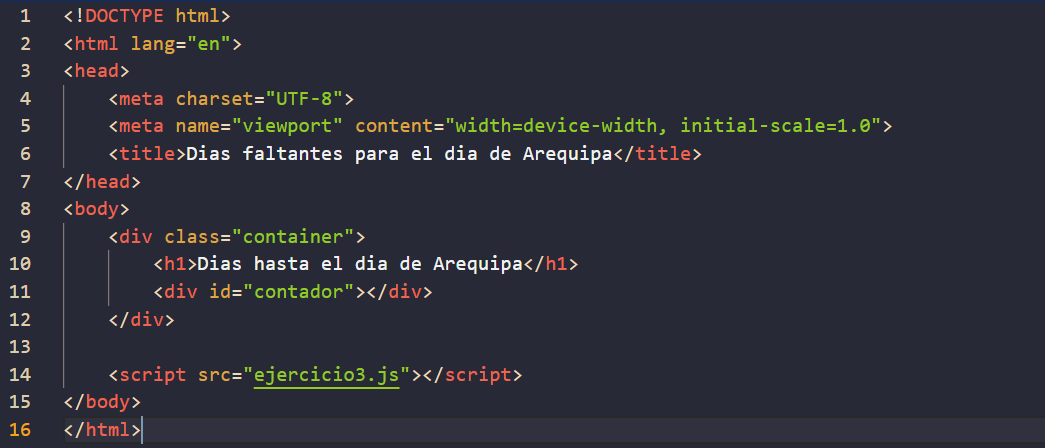
\includegraphics[width=1.0\textwidth, keepaspectratio]{img/ejercicio2a}
	\end{figure}
	\begin{itemize}
		\item JavaScript
	\end{itemize}
	\begin{figure}[H]
		\centering
		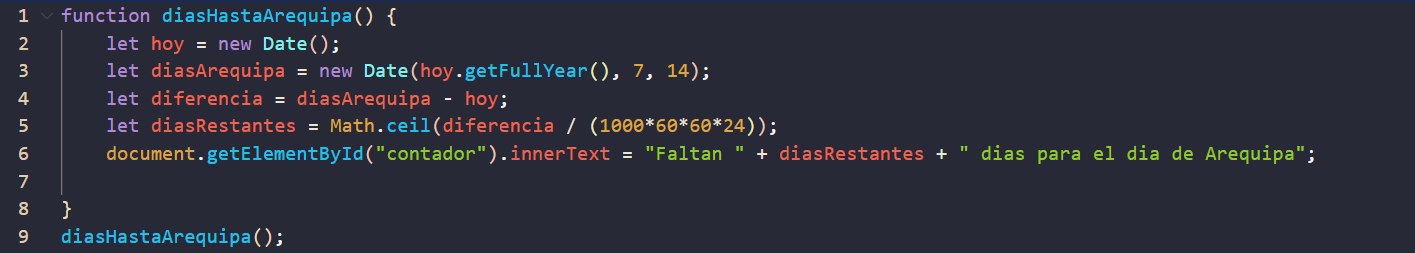
\includegraphics[width=1.0\textwidth, keepaspectratio]{img/ejercicio2b}
	\end{figure}
	\begin{itemize}
		\item Pagina
	\end{itemize}
	\begin{figure}[H]
		\centering
		
\includegraphics[width=1.0\textwidth, keepaspectratio]{img/ejercicio2c}
	\end{figure}
	
	\subsection{Ejercicio 3}
	\begin{itemize}
		\item HTML
	\end{itemize}
	\begin{figure}[H]
		\centering
		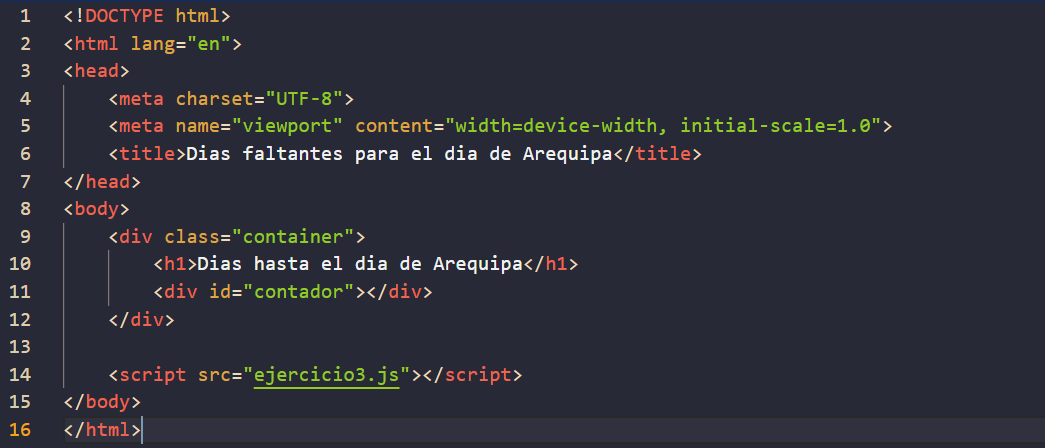
\includegraphics[width=1.0\textwidth, keepaspectratio]{img/ejercicio3a}
	\end{figure}
	\begin{itemize}
		\item JavaScript
	\end{itemize}
	\begin{figure}[H]
		\centering
		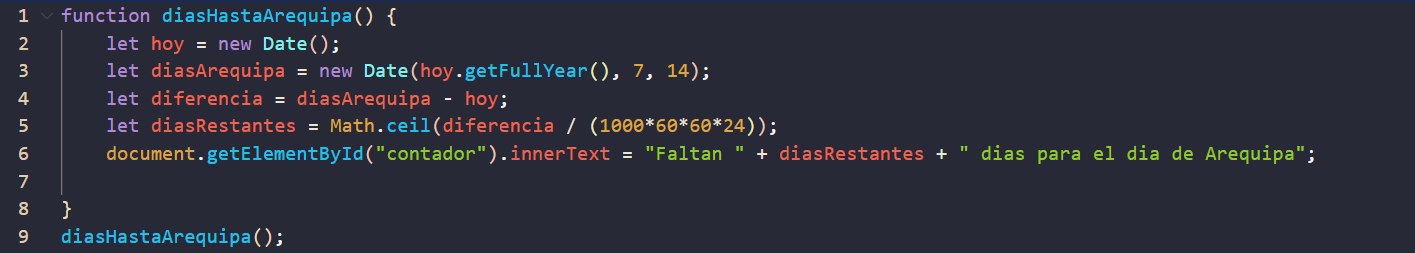
\includegraphics[width=1.0\textwidth, keepaspectratio]{img/ejercicio3b}
	\end{figure}
	\begin{itemize}
		\item Pagina
	\end{itemize}
	\begin{figure}[H]
		\centering
		
\includegraphics[width=1.0\textwidth, keepaspectratio]{img/ejercicio3c}
	\end{figure}
	
	\subsection{Ejercicio 4}
	\begin{itemize}
		\item HTML
	\end{itemize}
	\begin{figure}[H]
		\centering
		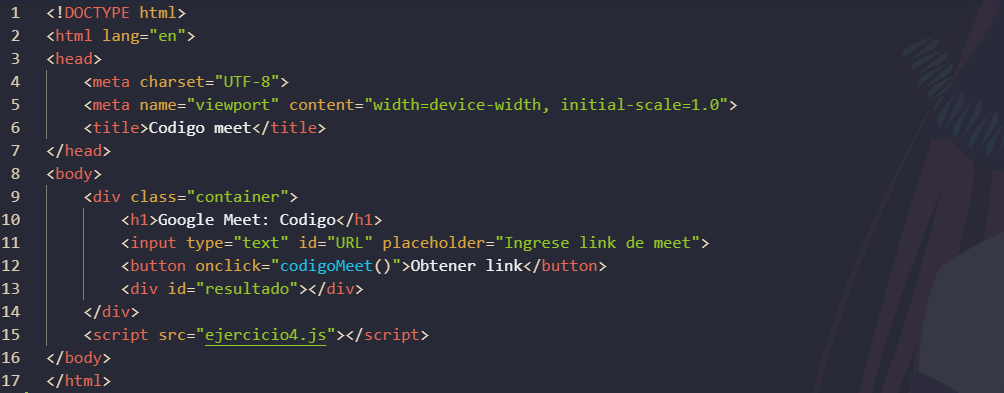
\includegraphics[width=1.0\textwidth, keepaspectratio]{img/ejercicio4a}
	\end{figure}
	\begin{itemize}
		\item JavaScript
	\end{itemize}
	\begin{figure}[H]
		\centering
		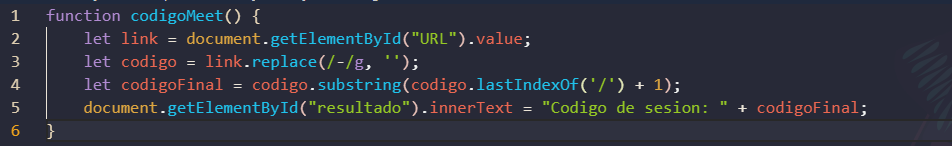
\includegraphics[width=1.0\textwidth, keepaspectratio]{img/ejercicio4b}
	\end{figure}
	\begin{itemize}
		\item Pagina
	\end{itemize}
	\begin{figure}[H]
		\centering
		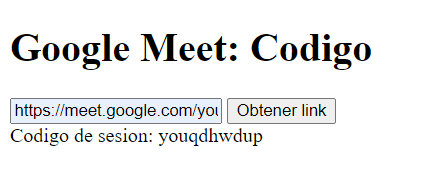
\includegraphics[width=1.0\textwidth, keepaspectratio]{img/ejercicio4c}
	\end{figure}
	
	\subsection{Ejercicio 5}
	\begin{itemize}
		\item HTML
	\end{itemize}
	\begin{figure}[H]
		\centering
		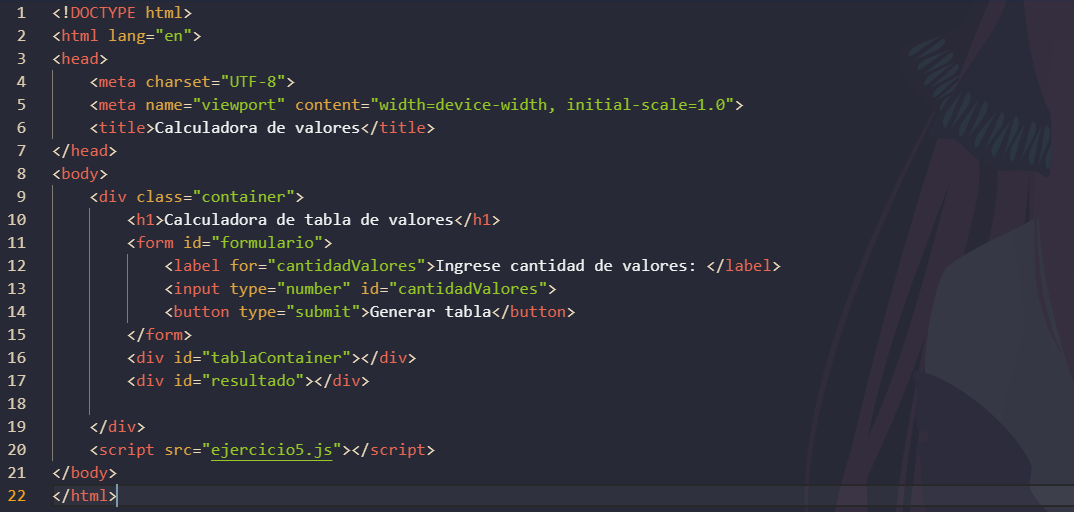
\includegraphics[width=1.0\textwidth, keepaspectratio]{img/ejercicio5a}
	\end{figure}
	\begin{itemize}
		\item JavaScript
	\end{itemize}
	\begin{figure}[H]
		\centering
		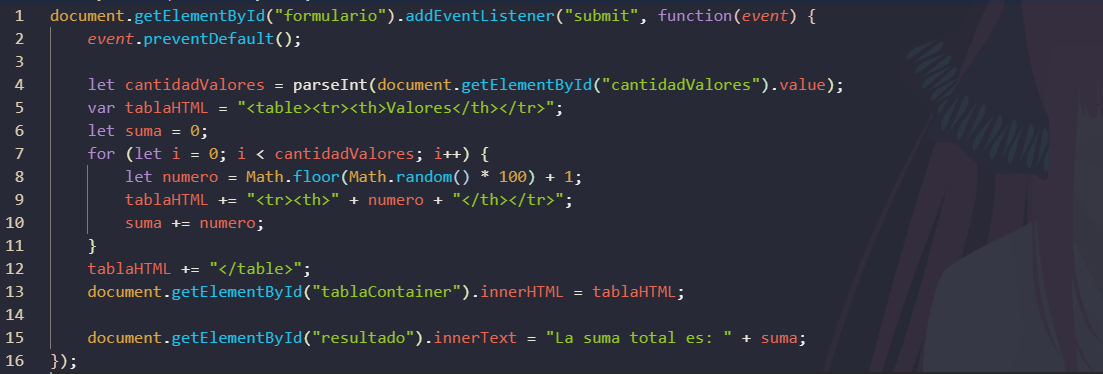
\includegraphics[width=1.0\textwidth, keepaspectratio]{img/ejercicio5b}
	\end{figure}
	\begin{itemize}
		\item Pagina
	\end{itemize}
	\begin{figure}[H]
		\centering
		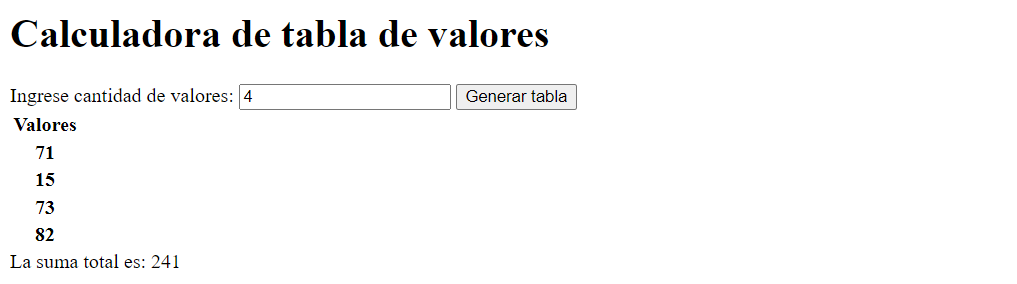
\includegraphics[width=1.0\textwidth, keepaspectratio]{img/ejercicio5c}
	\end{figure}
	
	\subsection{Ejercicio 6}
	\begin{itemize}
		\item Pagina 1 HTML
	\end{itemize}
	\begin{figure}[H]
		\centering
		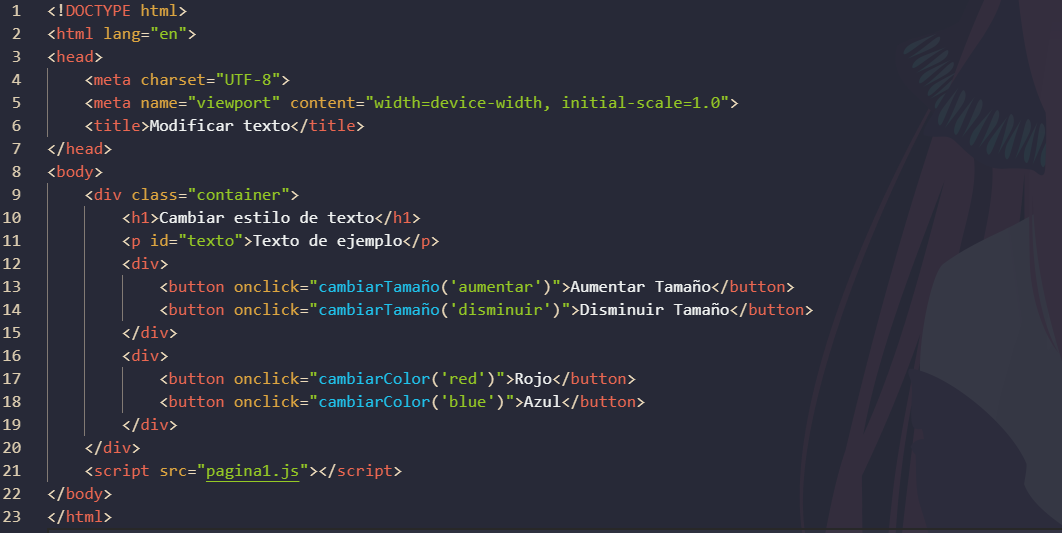
\includegraphics[width=1.0\textwidth, keepaspectratio]{img/pagina1a}
	\end{figure}
	\begin{itemize}
		\item Pagina 1 JavaScript
	\end{itemize}
	\begin{figure}[H]
		\centering
		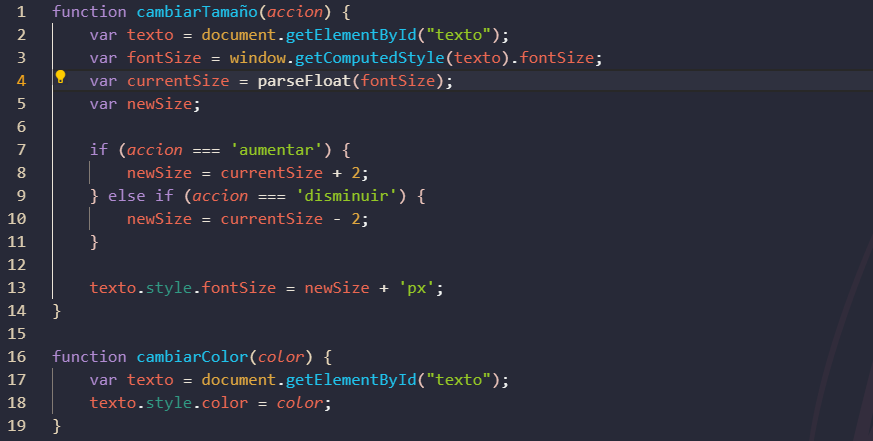
\includegraphics[width=1.0\textwidth, keepaspectratio]{img/pagina1b}
	\end{figure}
	\begin{itemize}
		\item Pagina 1
	\end{itemize}
	\begin{figure}[H]
		\centering
		
\includegraphics[width=1.0\textwidth, keepaspectratio]{img/pagina1c}
	\end{figure}
	\clearpage
	\begin{itemize}
		\item Pagina 2 HTML
	\end{itemize}
	\begin{figure}[H]
		\centering
		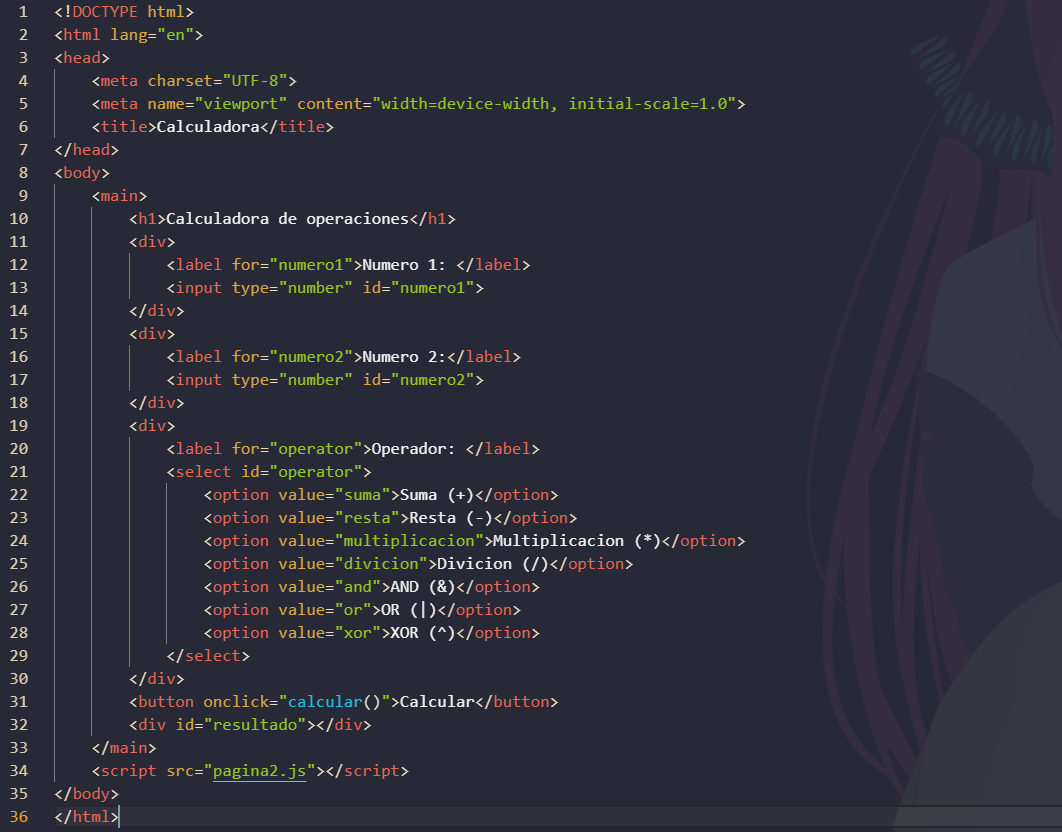
\includegraphics[width=1.0\textwidth, keepaspectratio]{img/pagina2a}
	\end{figure}
	\begin{itemize}
		\item Pagina 2 JavaScript
	\end{itemize}
	\begin{figure}[H]
		\centering
		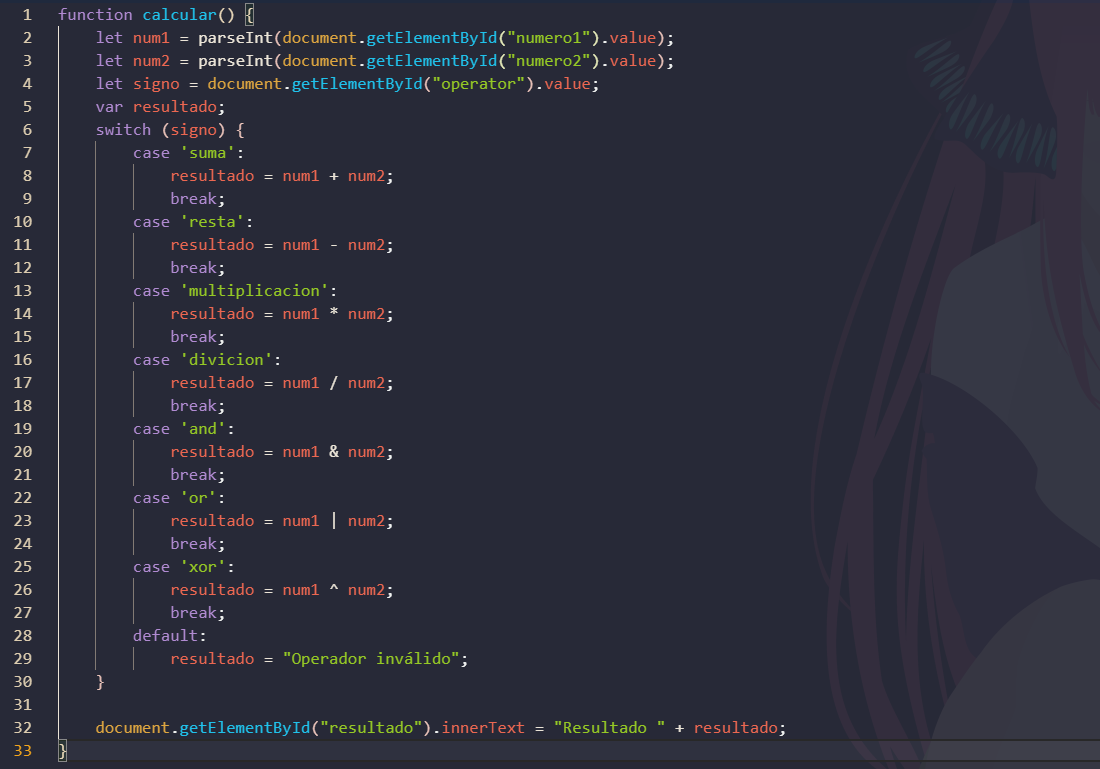
\includegraphics[width=1.0\textwidth, keepaspectratio]{img/pagina2b}
	\end{figure}
	\begin{itemize}
		\item Pagina 2
	\end{itemize}
	\begin{figure}[H]
		\centering
		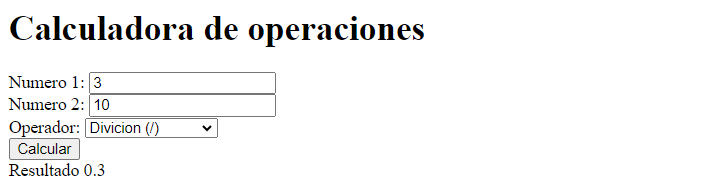
\includegraphics[width=1.0\textwidth, keepaspectratio]{img/pagina2c}
	\end{figure}
	
	
	
	\clearpage
	
	\section{Referencias}
	\begin{itemize}			
		\item \url{https://www.w3schools.com/js/default.asp}
	\end{itemize}	
	
	%\clearpage
	%\bibliographystyle{apalike}
	%\bibliographystyle{IEEEtranN}
	%\bibliography{bibliography}
	
\end{document}